\documentclass{../industrial-development}
\graphicspath{{01-business-processes/}}

\title{Бизнес-процессы компании по разработке программного обеспечения.
	Cхемы организации бизнеса по разработке ПО}
\author{Новиков Денис Александрович, \\Мехтиханов Леонид Игоревич, \\ПИ-21 МО}
\date{}

\begin{document}

\begin{frame}
  \titlepage
\end{frame}


\section{Ключевые задачи, стоящие перед компаниями и их реализация в бизнес-процессах}

\subsection{Понятие бизнес-процесса}


\begin{frame} \frametitle{Понятие бизнес-процесса}
	\begin{itemize}
		\item \alert{Бизнес-процесс} "--- логически завершенная цепочка взаимосвязанных и повторяющихся видов деятельности, в результате которых создается продукт (ПО) или сопутствующая услуга, предназначенная внутреннего или внешнего потребителя. Может являться частью другого, более общего бизнес-процесса.
		\item Потребителем результатов его деятельности может выступать другой бизнес-процесс.
	\end{itemize}
\end{frame}
\lecturenotes


\begin{frame} \frametitle{Преимущества процессного подхода}
	В отличие от иных форм моделирования, процессный подход нацелен на:
	\begin{itemize}
		\item удовлетворение требований клиента;
		\item снижение затрат на оперативное управление;
		\item анализ и выявление узких мест и резервов работы;
		\item снижение затрат на оперативное управление;
		\item создание эталонов, стандартов действий персонала;
		\item упрощение масштабирования бизнеса;
	\end{itemize}
\end{frame}
\lecturenotes


\subsection{Классификация бизнес-процессов}


\begin{frame} \frametitle{Классификация бизнес-процессов}
	По функциональному назначению бизнес-процессы разработки ПО делятся на:
	\begin{itemize}
		\item \alert{Основные} процессы
		\item \alert{Вспомогательные} процессы
		\item \alert{Управляющие} процессы
	\end{itemize}
\end{frame}
\lecturenotes


\begin{frame} \frametitle{Основные процессы}
	Направлены на непосредственно создание, эксплуатацию и поддержку ПО. Генерируют ценность для клиента и прибыль для компании.
	
	\begin{block}{Включают в себя}
		\begin{itemize}
			\item анализ потребностей клиента
			\item формирование требований к ПО
			\item разработку ПО
			\item поддержку и сопровождение продукта
		\end{itemize}
	\end{block}
	\begin{block}{Результат}
		ПО или услуга удовлетворяющее потребностям заказчика.
	\end{block}
\end{frame}
\lecturenotes


\begin{frame} \frametitle{Вспомогательные процессы}
	Обеспечивают ресурсы для основных процессов. Не создают продукт напрямую, но необходимы для его создания.

	\begin{block}{Включают в себя}
		\begin{itemize}
			\item поиск и подготовку кадров
			\item организацию технической и иной инфраструктуры
			\item организацию труда персонала, в т.ч. оснащение рабочих мест
		\end{itemize}
	\end{block}
	\begin{block}{Результат}
		Ресурсы, необходимые для функционирования основных процессов (разработка и сопровождение ПО).
	\end{block}
\end{frame}
\lecturenotes


\begin{frame} \frametitle{Управляющие процессы}
	Обеспечивают координацию и слаженную работу бизнес-процессов и функциональных единиц компании, ее ориентацию на рынке разработки ПО.
	
	\begin{block}{Включают в себя}
		\begin{itemize}
		\item планирование
		\item коммуникации (разъяснения, мотивация и поддержка сотрудников)
		\item реализацию, контроль выполнения и корректировку плана действий
		\item оценку результатов
		\end{itemize}
	\end{block}
	\begin{block}{Результат}
		Организационная структура и управленческие решения, обеспечивающие функционирование компании.
	\end{block}
\end{frame}
\lecturenotes


\subsection{Жизненный цикл программного обеспечения}


\begin{frame} \frametitle{Жизненный цикл ПО}
	\begin{itemize}
		\item \alert{Жизненный цикл} "--- это условная схема, включающая отдельные этапы, которые представляют стадии процесса создания и эксплуатации ПО.
		\item \alert{Жизненный цикл} начинается на этапе анализа и формирования требований к продукту, заканчивается в момент выведения из эксплуатации.
		\item \alert{Жизненный цикл} ПО обусловливает содержание и последовательность основных бизнес-процессов
	\end{itemize}
\end{frame}
\lecturenotes


\begin{frame} \frametitle{Основные этапы жизненного цикла}
	\centerline{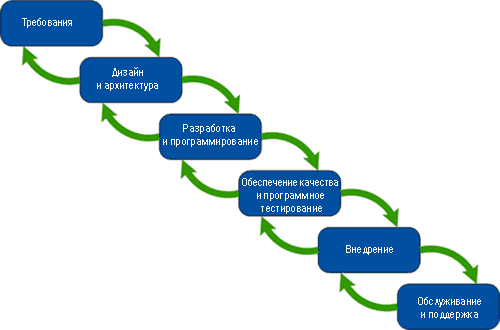
\includegraphics[height=0.70\textheight]{image15.png}}	
\end{frame}
\lecturenotes


\subsection{Модели жизненного цикла}


\begin{frame} \frametitle{Модель жизненного цикла ПО}
	\alert{Модель жизненного цикла} "--- шаблон этапов разработки ПО, предназначенный для оптимизации проектирования и создания качественного ПО.
	
	Это методология, определяющая процессы и средства, необходимые для успешного завершения проекта.
	
	\centerline{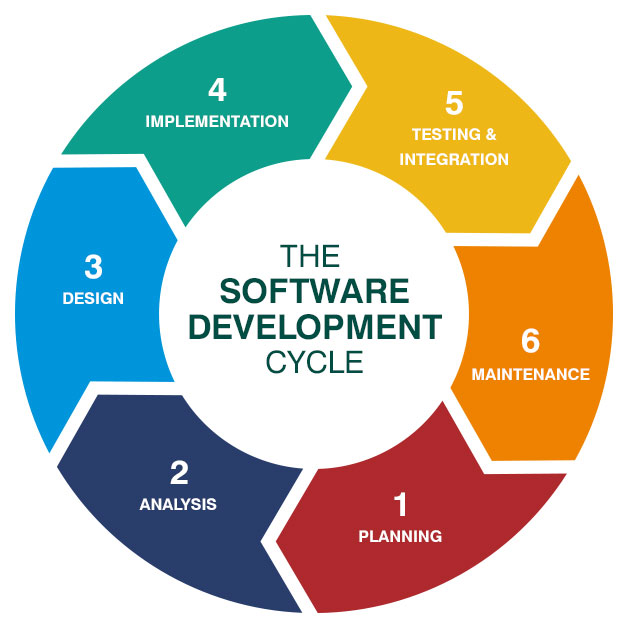
\includegraphics[height=0.50\textheight]{image14.png}}
\end{frame}
\lecturenotes


\begin{frame} \frametitle{Модели жизненного цикла. Водопад}
	\alert{Водопад (каскадный)} "--- модель, в которой разработка состоит из последовательных фаз анализа требований, проектирования, реализации, тестирования, интеграции и поддержки. Переход между фазами происходит только после полного завершения предыдущей фазы.
	
	\centerline{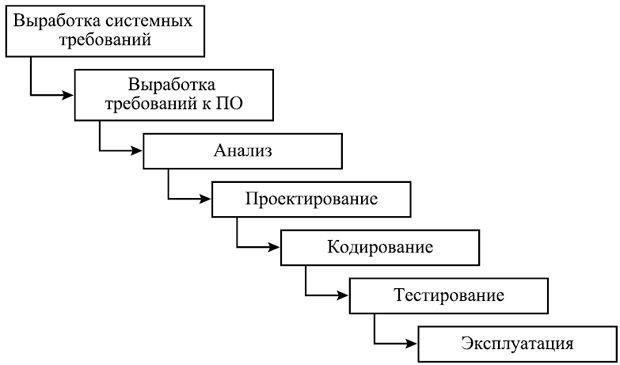
\includegraphics[height=0.50\textheight]{image16.png}}
\end{frame}
\lecturenotes


\begin{frame} \frametitle{Модели жизненного цикла. Итеративный подход}
	\alert{Итеративный подход} "--- предусматривает выполнение работ параллельно с анализом полученных результатов и корректировкой этапов работы.
	
	Проект многократно проходит повторяющийся цикл PDCA: Plan "--- Do "--- Check "--- Act (Планирование "--- Реализация "--- Проверка "--- Оценка).
	
	\centerline{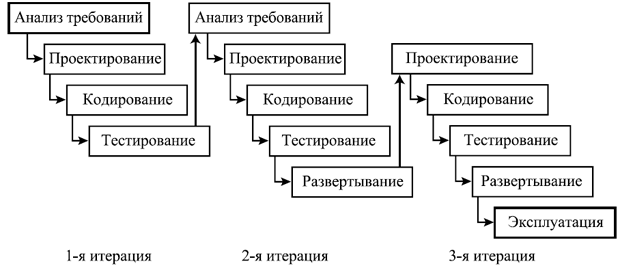
\includegraphics[height=0.50\textheight]{image12.png}}
\end{frame}
\lecturenotes


\begin{frame} \frametitle{Модели жизненного цикла. Agile}
	\alert{Гибкая методология разработки} (agile software development) "--- нацелена на минимизацию рисков путём сведения разработки к серии коротких циклов (итераций), продолжительностью две-три недели, после каждой из которых заказчик может наблюдать результат и понять, удовлетворяет он его или нет.
	
	\centerline{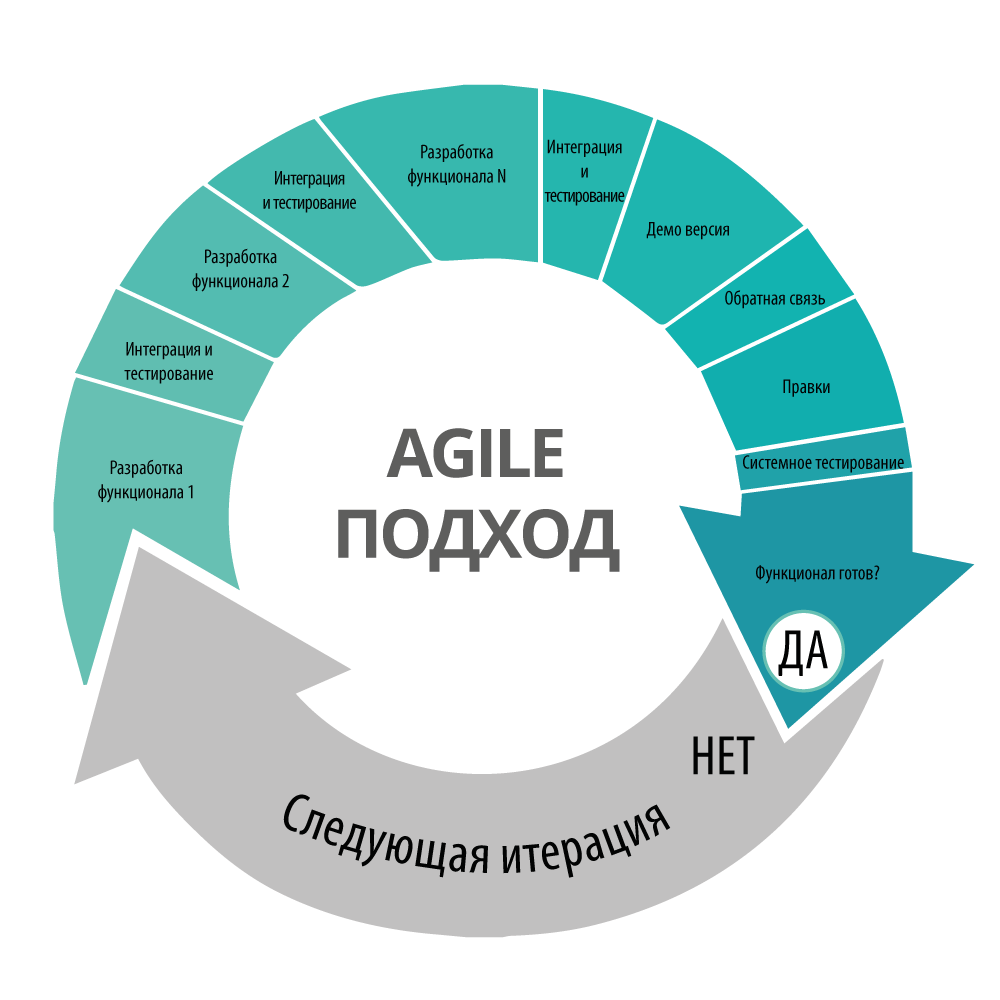
\includegraphics[height=0.50\textheight]{image18.png}}
\end{frame}
\lecturenotes


\subsection{Бизнес-процессы создания ПО}


\begin{frame} \frametitle{Бизнес-процессы создания ПО. Подготовка}
	\begin{itemize}
		\item Бизнес-процесс подготовки является необязательным и в ряде случаев является частью бизнес-процесса анализа.
		\item Применяется в случаях когда затраты на более строгий анализ слишком высоки, позволяет отказаться от нереализуемых и потенциально невостребованных продуктов на ранних этапах.
	\end{itemize}
\end{frame}
\lecturenotes


\begin{frame} \frametitle{Бизнес-процессы создания ПО. Подготовка}
	\begin{block}{Предназначен для анализа}
		\begin{itemize}
			\item целей на основе исходной идеи
			\item востребованности будущего продукта
			\item рисков
			\item предварительного технического решения
			\item трудозатрат и необходимых ресурсов
			\item реализуемости
		\end{itemize}
	\end{block}
	\begin{block}{Результат}
		Решение, о том, стоит ли продолжать работы.
	\end{block}
\end{frame}
\lecturenotes


\begin{frame} \frametitle{Бизнес-процессы создания ПО. Анализ и проектирование}
	%\centerline{
\includegraphics[height=0.10\textheight]{image6.png}}
	\begin{block}{Предназначен для}
		\begin{itemize}
			\item определения потребностей клиента и путей их удовлетворения
			\item оценки существующих решений, их соответствия поставленной задаче
			\item разработки архитектуры решения, определение используемых технологий
			\item формирования технического задания, спецификации
		\end{itemize}
	\end{block}
	\begin{block}{Результат}
		Формальные требования к разрабатываемому ПО, технический проект (техническое задание).
	\end{block}
\end{frame}
\lecturenotes


\begin{frame} \frametitle{Бизнес-процессы создания ПО. Планирование}
	%\centerline{
\includegraphics[height=0.10\textheight]{image17.png}}
	\begin{block}{Предназначен для}
		\begin{itemize}
			\item формирования оптимального плана работ, выделение основных этапов, условий их завершений
			\item оценки временных и стоимостных затрат при различных подходах, с учетом доступных ресурсов
		\end{itemize}
	\end{block}
	\begin{block}{Результат}
		Целевой план работ, план бюджетирования.
	\end{block}
\end{frame}
\lecturenotes


\begin{frame} \frametitle{Бизнес-процессы создания ПО. Технико-экономического обоснование}
	%\centerline{
\includegraphics[height=0.10\textheight]{image13.png}}
	\begin{block}{Предназначен для}
		\begin{itemize}
			\item определения эффект от внедрения, его оценки с учетом предполагаемого срока эксплуатации
			\item оценки рентабельности инвестиций. Например, путем расчета соотношения эффект / затраты
			\item планирования бюджетирования
		\end{itemize}
	\end{block}
	\begin{block}{Результат}
		Оценка экономического эффекта, определение необходимости дальнейшей работы над проектом.
	\end{block}
\end{frame}
\lecturenotes


\begin{frame} \frametitle{Бизнес-процессы создания ПО. Разработка}
	\begin{block}{Предназначен для}
		\begin{itemize}
			\item реализации архитектуры проекта
			\item реализации функционала ПО в соответствии со спецификацией. техническим заданием
			\item разработки документации
		\end{itemize}
	\end{block}
	\begin{block}{Результат}
		Программное обеспечение.
	\end{block}
\end{frame}
\lecturenotes


\begin{frame} \frametitle{Бизнес-процессы создания ПО. Контроль качества}
	\begin{itemize}
		\item Качество ПО (Software Quality) "--- это степень, в которой программное обеспечение обладает требуемой комбинацией свойств. [1061-1998 IEEE Standard for Software Quality Metrics Methodology]
		\item Качество ПО (Software Quality) "--- это совокупность характеристик программного обеспечения, относящихся к его способности удовлетворять установленные и предполагаемые потребности. [ISO 8402:1994 Quality management and quality assurance]
	\end{itemize}
\end{frame}
\lecturenotes


\begin{frame} \frametitle{Бизнес-процессы создания ПО. Контроль качества}
	\begin{itemize}
		\item Обеспечение качества (Quality Assurance) "--- это совокупность мероприятий, предпринимаемых на разных стадиях жизненного цикла ПО для обеспечения требуемого уровня качества выпускаемого продукта.
		\item Контроль качества (Quality Control) "--- это совокупность действий, для получения информации о актуальном состоянии ПО в разрезах: "готовность продукта к выпуску", "соответствие зафиксированным требованиям", "соответствие заявленному уровню качества продукта".
	\end{itemize}
\end{frame}
\lecturenotes


\begin{frame} \frametitle{Бизнес-процессы создания ПО. Контроль качества}
	\begin{block}{Предназначен для}
		\begin{itemize}
			\item проверки корректности реализации, соответствия спецификации и техническому заданию
			\item проверки соответствия тестовых показателей нормативам, анализ их динамики
			\item контроля качества программного кода
			\item контроля актуальности документации
		\end{itemize}
	\end{block}
	\begin{block}{Результат}
		Информация о фактическом состоянии продукта, мере его соответствия целевым показателям.
	\end{block}
\end{frame}
\lecturenotes


\begin{frame} \frametitle{Бизнес-процессы создания ПО. Внедрение}
	\begin{block}{Предназначен для}
		\begin{itemize}
			\item финальной проверки продукта на соответствие спецификации
			\item проведения приемочных испытаний ПО
			\item передача ПО и документации заказчику
		\end{itemize}
	\end{block}
	\begin{block}{Результат}
		Запуск системы в реальных условиях.
	\end{block}
\end{frame}
\lecturenotes


\begin{frame} \frametitle{Бизнес-процессы создания ПО. Эксплуатация}
	\begin{block}{Предназначен для}
		\begin{itemize}
			\item извлечения ценности из продукта заказчиком
			\item получения обратной связи, перехода к процессу разработки при необходимости
			\item завершения в случае, когда ПО перестает удовлетворять требованиям заказчика
		\end{itemize}
	\end{block}
	\begin{block}{Результат}
		Эксплуатация в реальных условиях, выполнение бизнес-функций заказчика.
	\end{block}
\end{frame}
\lecturenotes


\begin{frame} \frametitle{Бизнес-процессы создания ПО. Завершение эксплуатации}
	\begin{itemize}
		\item Происходит когда продукт не удовлетворяет требованиям заказчика и его доработка невозможна или нерентабельна.
		\item Это может произойти по ряду причин: изменение потребностей бизнеса, конъюнктуры рынка, технологические изменения.
	\end{itemize}
\end{frame}
\lecturenotes


\begin{frame} \frametitle{Бизнес-процессы создания ПО. Завершение эксплуатации}
	\begin{block}{Предназначен для}
		\begin{itemize}
			\item анализа опыта с целью оптимизации бизнес-процессов создания ПО
			\item завершения работы над проектом и остановки сопровождения
		\end{itemize}
	\end{block}
	\begin{block}{Результат}
		Полное прекращение деятельности в рамках проекта.
	\end{block}
\end{frame}
\lecturenotes


\section{Типичные схемы организации бизнеса по разработке}

\subsection{Разработка собственного продукта}

\subsection{Разработка продукта на заказ}

\subsection{Аутсорсинг}

\subsection{ИТ-консалтинг}


%\begin{frame} \frametitle{Пример слайда}
%  \begin{block}{Важный факт}
%    Промышленная разработка является коллективным процессом\dots
%  \end{block}
%  
%  \begin{itemize}
%  \item Тезис 1\dots
%  \item Тезис 2\dots
%  \item Важный текст на слайдах можно \alert{выделять}\dots
%  \end{itemize}
%\end{frame}
%\lecturenotes
%Текст конспекта, относящийся к слайду с указанием источника~\cite[с.~97--99]{Brooks}.
%На интернет-источники можно ссылаться не по ГОСТу, но с обязательной гиперссылкой~\cite{Fowler}.


%\begin{thebibliography}{99}
%\bibitem{Brooks} Брукс Ф. Мифический человеко-месяц или как создаются программные системы. СПб~: Символ-плюс, 2000.
%\bibitem{Fowler} \href{https://martinfowler.com/articles/injection.html}{Fowler M. Inversion of Control Containers and the Dependency Injection pattern.}
%\end{thebibliography}

\end{document}

%%% Local Variables: 
%%% mode: TeX-pdf
%%% TeX-master: t
%%% End: 
